\section{Representación de Superficies}
\label{sec:surface_rep}

\begin{wrapfigure}[11]{l}{0.4\linewidth}
	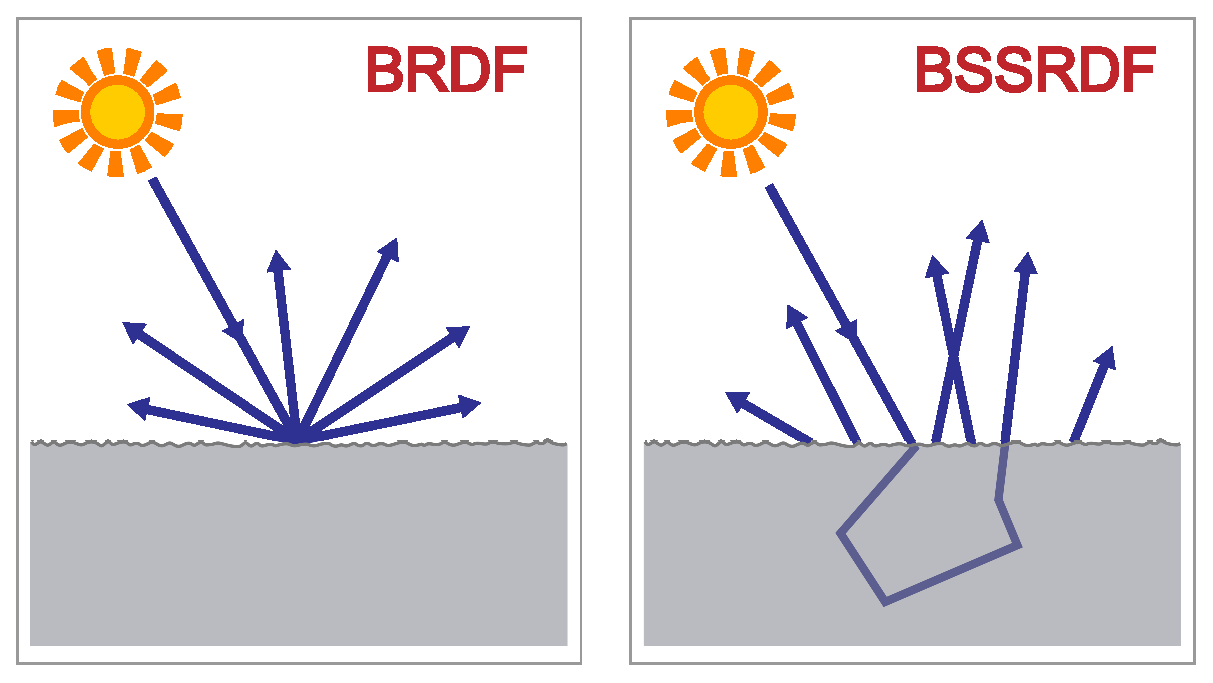
\includegraphics[width=\linewidth]{media/brdf_vs.eps}
	\caption
	{
    	BRDF izquierda, punto de salida es igual al punto de entrada.\\ 
    	BSSRDF derecha, se observa como el punto de salida es distinto al de entrada.
	}
	\label{fig:bssrdf}
\end{wrapfigure}

Los materiales interaccionan con la luz de distintas maneras. Esto hace que la apariencia de ciertos materiales difiera según la condiciones de la luz en una escena. Algunos materiales parecen espejos mientras que otros son totalmente difusos. Son visualmente distinguible materiales como vidrio, madera o metales. Las propiedades de reflectancia de una superficie afectan la apariencia del objeto \cite{advanced_gi2006}, estos objetos se distinguen por la cantidad de luz reflectada en ciertas direcciones. 

En el caso más general, un rayo de luz entra en algún punto $p$ sobre una superficie en una escena, este rayo de luz tiene una dirección incidente $\Psi$ y puede salir de esta superficie sobre otro punto $q$ con dirección saliente $\Theta$. La función que define esta relación entre la radiancia incidente y la radiancia reflectada se llama \ac{BSSRDF}.

\subsection{Función de Distribución de Reflectancia Bidireccional}
Al asumir que la luz incidente en algún punto $x$ sale del mismo punto $x$ (ignorando la transluminiscencia) las propiedades de reflectancia de una superficie son entonces descritas por una \ac{BRDF}.

La \ac{BRDF} en un punto $x$ se define entonces como la distribución de la radiancia reflectada diferencial en una dirección saliente $\Theta$ y la irradiancia incidente diferencial a través de un ángulo solido $dw_{\Psi}$. La función \ac{BRDF} puede ser escrita de la siguiente forma \cite{advanced_gi2006}:

\begin{equation}
	\begin{split}
        f_{r}(x, \Psi\to\Theta) &= \frac{dL(x\to\Theta)}{dE(x\gets\Psi)}\\
        &= \frac{dL(x\to\Theta)}{L(x\gets\Psi)\cos(N_{x}, \Psi)dw_{\Psi}}
	\end{split}
	\label{eq:brdf_def}
\end{equation}

Donde $\cos(N_{x}, \Psi)$ es el coseno del ángulo formado entre la normal en el punto $x$ y el vector dirección $\Psi$

\subsubsection{Propiedades de la Función BRDF}

La función BRDF tiene una variada cantidad de importantes propiedades:

\begin{enumerate}
	\item Dimensión: La función BRDF es una función cuatridimensional definida sobre cada punto de una superficie, dos dimensiones corresponden a la dirección entrante y dos a la dirección saliente.
	\item Reciprocidad: El resultado de la función BRDF es el mismo si se intercambian la dirección entrante y la dirección saliente:
    	\begin{equation}
            f_{r}(x, \Psi\to\Theta) = f_{r}(x, \Theta\to\Psi)
    	\end{equation}
	\item Conservación de la energía: La ley de conservación de la energía dicta que la cantidad total de energía reflectada en todas las direcciones debe ser menor o igual a la cantidad de total de energía incidente sobre las superficies: 
    	\begin{equation}
    		\int_{\Omega^{+}}f_{r}(x, \Psi\to\Theta)\cos(N_{x}, \Theta)dw_{\Theta} \leq 1
    	\end{equation}
\end{enumerate}

\subsubsection{Ejemplos de BRDF}
Dependiendo del comportamiento de la \ac{BRDF}, el material se verá como una superficie difusa, como un espejo o como una mezcla de ambos (lustroso o \emph{glossy}). Los tipos de BRDF relevantes para este trabajo serán listados aquí.

\begin{figure}[H]
	\centering
	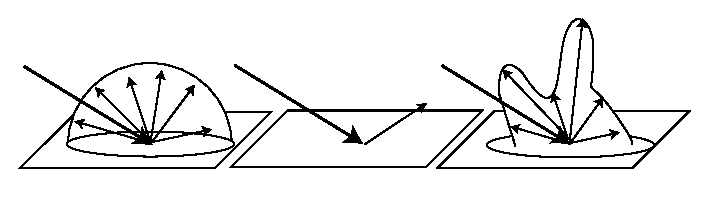
\includegraphics[width=0.85\linewidth]{media/brdfs_types.eps}
	\caption{Ejemplos de superficies: totalmente difusa izquierda, totalmente especular centro, lustrosa (\emph{glossy}) derecha \cite{advanced_gi2006}.}
	\label{fig:brdf_types}
\end{figure}

\paragraph{Superficies Difusas:}
Algunos materiales reflectan la luz de forma uniforme sobre la totalidad de la semiesfera de reflectancia. Esto quiere decir que según la distribución de la irradiancia, la radiancia reflectada es independiente de la dirección de salida. Estos materiales son llamados reflectores difusos y el valor de su \ac{BRDF} es una constante para todos los valores $\Theta$ y $\Psi$. Para un observador un punto sobre una superficie difusa se ve igual desde todas las direcciones \cite{advanced_gi2006}. Para una superficie difusa ideal, la reflexión difusa puede ser representada como:

\begin{equation}
    f_{r}(x, \Psi\leftrightarrow\Theta) = \frac{\rho_{d}}{\pi}
    \label{eq:diffuse_reflection}
\end{equation}

La reflectancia $\rho_{d}$ representa la fracción de la energía incidente que es reflectada en la superficie. Para materiales físicamente correctos, $\rho_{d}$ varía entre 0 y 1.

\paragraph{Superficies Especulares:}
\label{para:speculars}
Superficies especulares perfectas solo reflejan o refractan luz en una dirección específica.
\paragraph{Reflexión Especular:}
La dirección de reflexión puede ser obtenida utilizando la ley de reflexión, esta indica que la dirección de la luz incidente y saliente tienen un ángulo equivalente con la normal de la superficie. Dado que la luz es incidente con respecto a la superficie con vector dirección $\Psi$, y la normal de la superficie es $N$, la luz incidente es reflectada en la dirección $R$:

\begin{equation}
    R = 2(N\cdot\Psi)N - \Psi
    \label{eq:reflectance_direction}
\end{equation}

Un reflector especular perfecto tiene solo una dirección de salida donde la \ac{BRDF} es diferente de $0$, esto implica que el valor de la \ac{BRDF} en esa dirección es infinito.

\paragraph{Superficies Lustrosas:}
La mayoría de las superficies no son ni idealmente difusas ni idealmente especulares, sino que demuestran una combinación de ambas características de reflectancia. Estas superficies son llamadas superficies lustrosas o superficies \emph{glossy}. La \ac{BRDF} que describe esta clase de materiales es usualmente difícil de modelar de forma analítica \cite{advanced_gi2006}.

\subsubsection{Modelos de sombreado.}
Materiales reales puede tener \ac{BRDF}s particularmente complejas. En computación gráfica existen varios modelos que intentan capturar la complejidad de las \ac{BRDF}s. En la siguiente sección se expande sobre ciertos modelos relevantes a este trabajo. Nótese que $\Psi$ es la dirección de la luz (dirección incidente), $\Theta$ es la dirección del observador (dirección saliente) y $N$ la normal de la superficie.

\paragraph{Modelo de Lambert:}
Uno de los modelos más simples, este modelo es ideal para superficies difusas, en este modelo la \ac{BRDF} es una constante como ya fue descrito anteriormente en la ecuación \ref{eq:diffuse_reflection}.

\begin{equation}
    f_{r}(x, \Psi\leftrightarrow\Theta) = k_{d} = \frac{\rho_{d}}{\pi}
    \label{eq:lambert}
\end{equation}

Donde $\rho_{d}$ es la reflexión difusa.

\paragraph{Modelo de Phong:}
La \ac{BRDF} del modelo de Phong es:

\begin{equation}
    f_{r}(x, \Psi\leftrightarrow\Theta) = k_{s}\frac{(R\cdot \Theta)^n}{N\cdot\Psi} + k_{d}
    \label{eq:phong}
\end{equation}

Donde el vector reflectado $R$ es calculado con la ecuación \ref{eq:reflectance_direction}.

\paragraph{Modelo de Blinn-Phong:}
\label{para:blinn_phong}
El modelo Blinn-Phong utiliza el vector medio $H$ entre $\Psi$ y $\Theta$ de la siguiente manera:

\begin{equation}
    f_{r}(x, \Psi\leftrightarrow\Theta) = k_{s}\frac{(N\cdot H)^n}{N\cdot\Psi} + k_{d}
    \label{eq:blinn_phong_pr}
\end{equation}

El valor $n$ varía según las propiedades del material. Un mayor valor provee un lóbulo especular más pequeño, simulando superficies lisas y pulidas.

\begin{figure}[H]
	\centering
	\begin{subfigure}[t]{0.25\textwidth}
		\centering
		\captionsetup{justification=centering}
		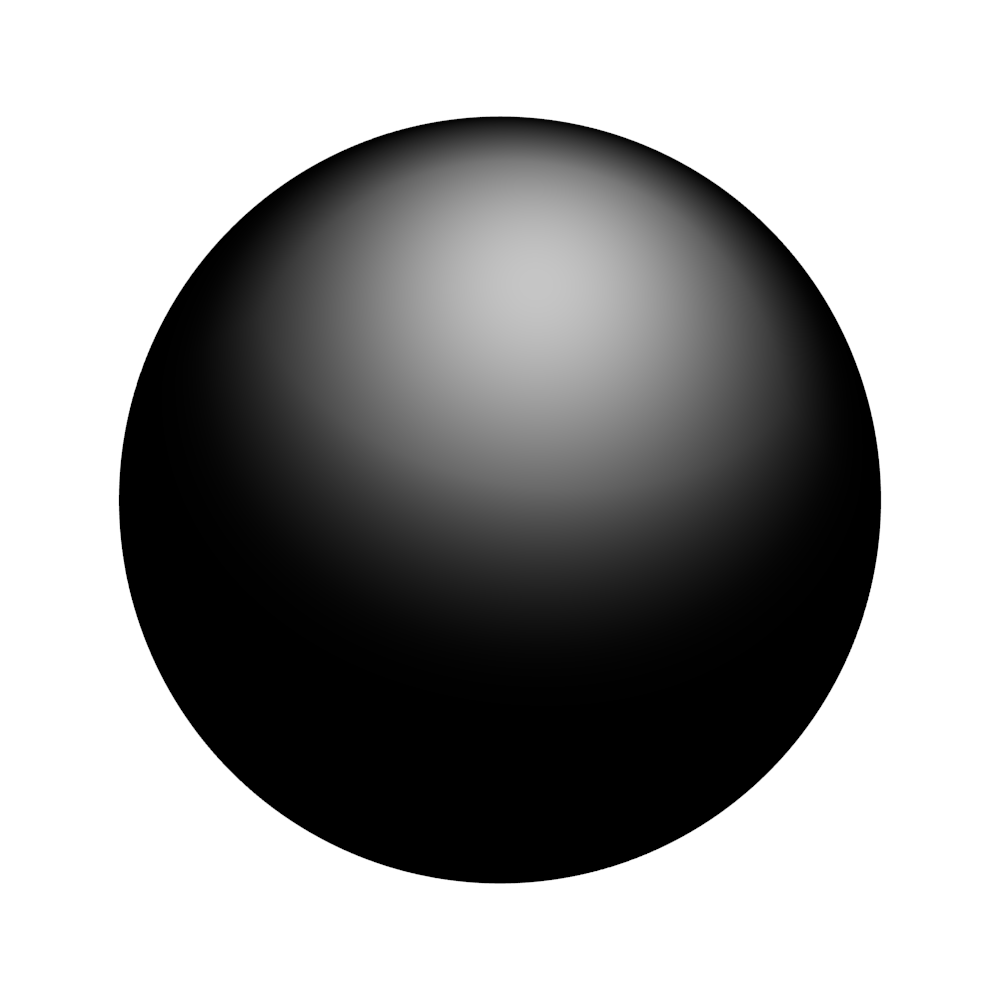
\includegraphics[width=\linewidth]{media/blinn_10.png}
		\caption*{$n = 10$}
	\end{subfigure}%
	\begin{subfigure}[t]{0.25\textwidth}
		\centering
		\captionsetup{justification=centering}
		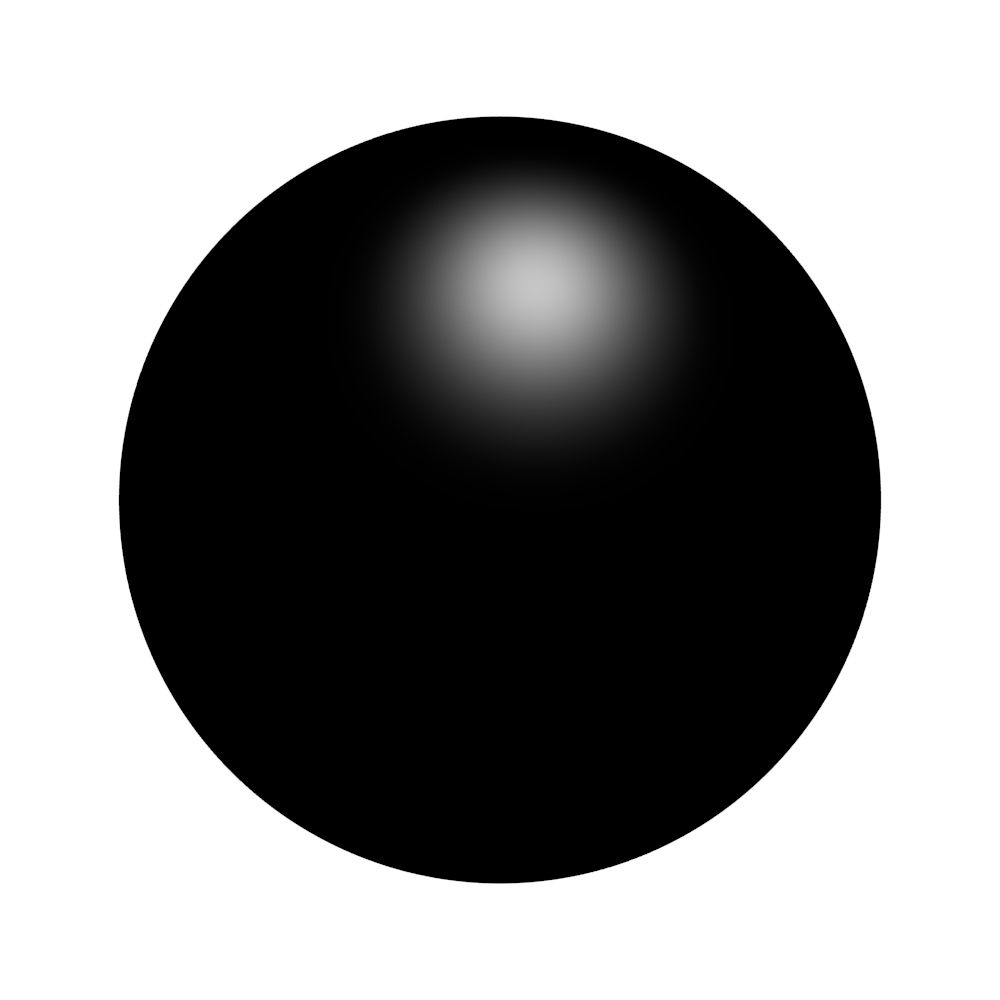
\includegraphics[width=\linewidth]{media/blinn_50.png}
		\caption*{$n = 50$}
	\end{subfigure}%
	\begin{subfigure}[t]{0.25\textwidth}
		\centering
		\captionsetup{justification=centering}
		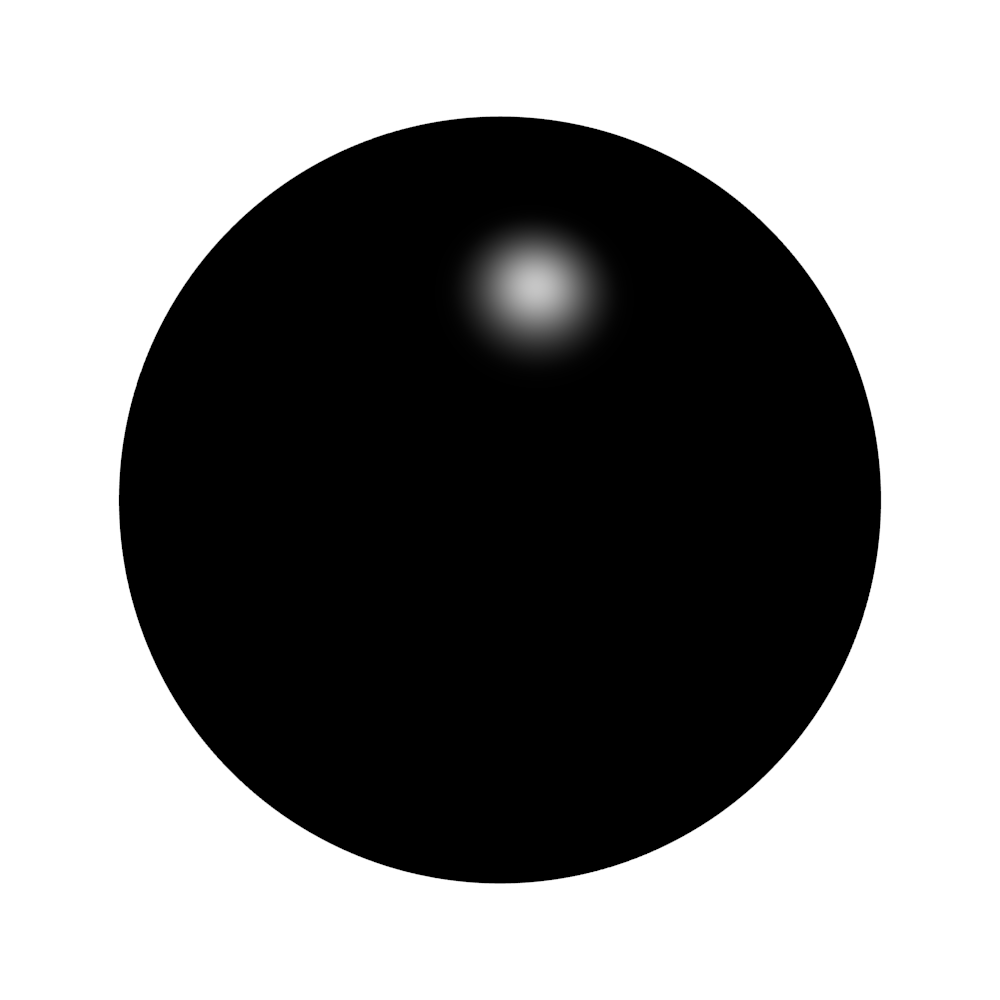
\includegraphics[width=\linewidth]{media/blinn_150.png}
		\caption*{$n = 150$}
	\end{subfigure}%
	\begin{subfigure}[t]{0.25\textwidth}
		\centering
		\captionsetup{justification=centering}
		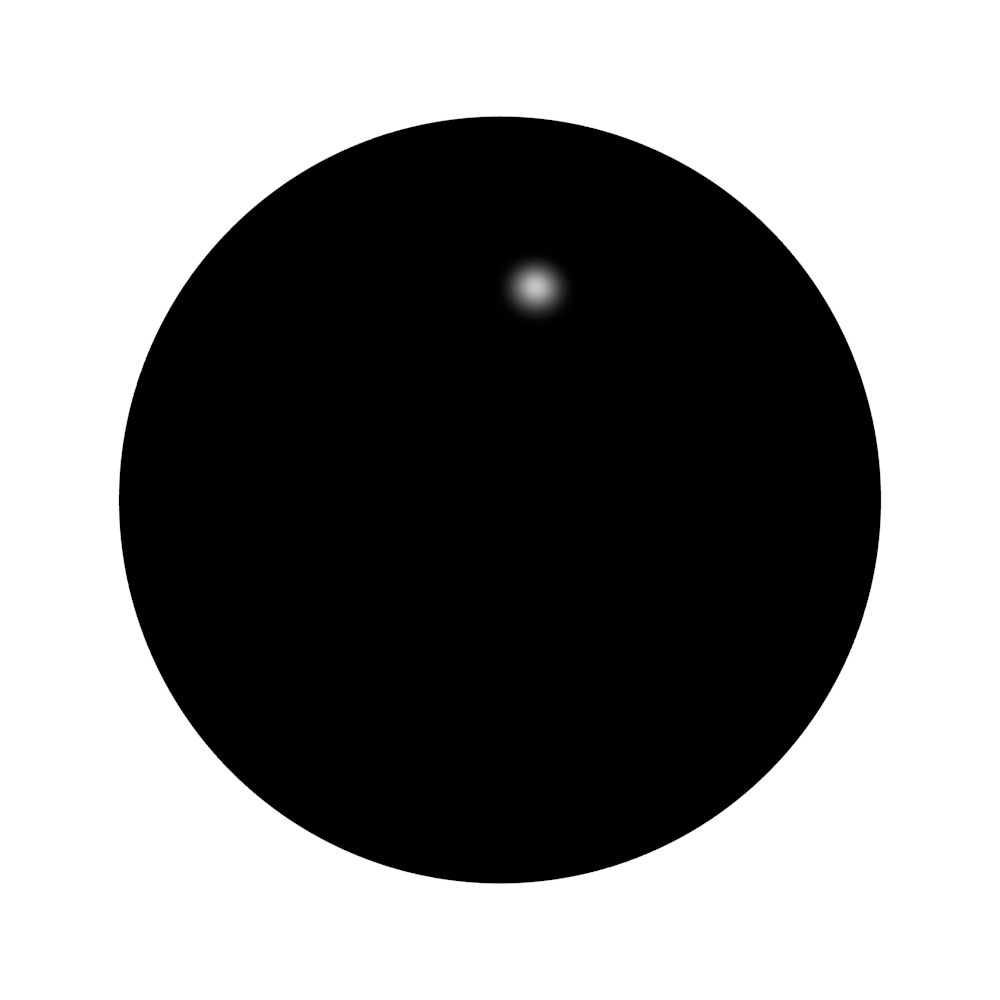
\includegraphics[width=\linewidth]{media/blinn_350.png}
		\caption*{$n = 350$}
	\end{subfigure}%
	\caption{Distribución especular para distintos valores de $n$ en el modelo Blinn-Phong.}
	\label{fig:blinn_spec_comparison}
\end{figure}

\paragraph{Modelo de Blinn-Phong Modificado:}
\label{para:blinn_phong_mod}
El modelo de Phong a pesar de ser simple este tiene ciertas limitaciones, no es ni conservador de energía ni reciproco y tiene problemas para simular materiales reales. El modelo modificado toma en cuenta algunos de estos problemas:

\begin{equation}
    f_{r}(x, \Psi\leftrightarrow\Theta) = k_{s}(N\cdot H)^n + k_{d}
    \label{eq:blinn_phong}
\end{equation}

\begin{figure}[H]
	\centering
	\begin{subfigure}[t]{0.33\textwidth}
		\centering
		\captionsetup{justification=centering}
		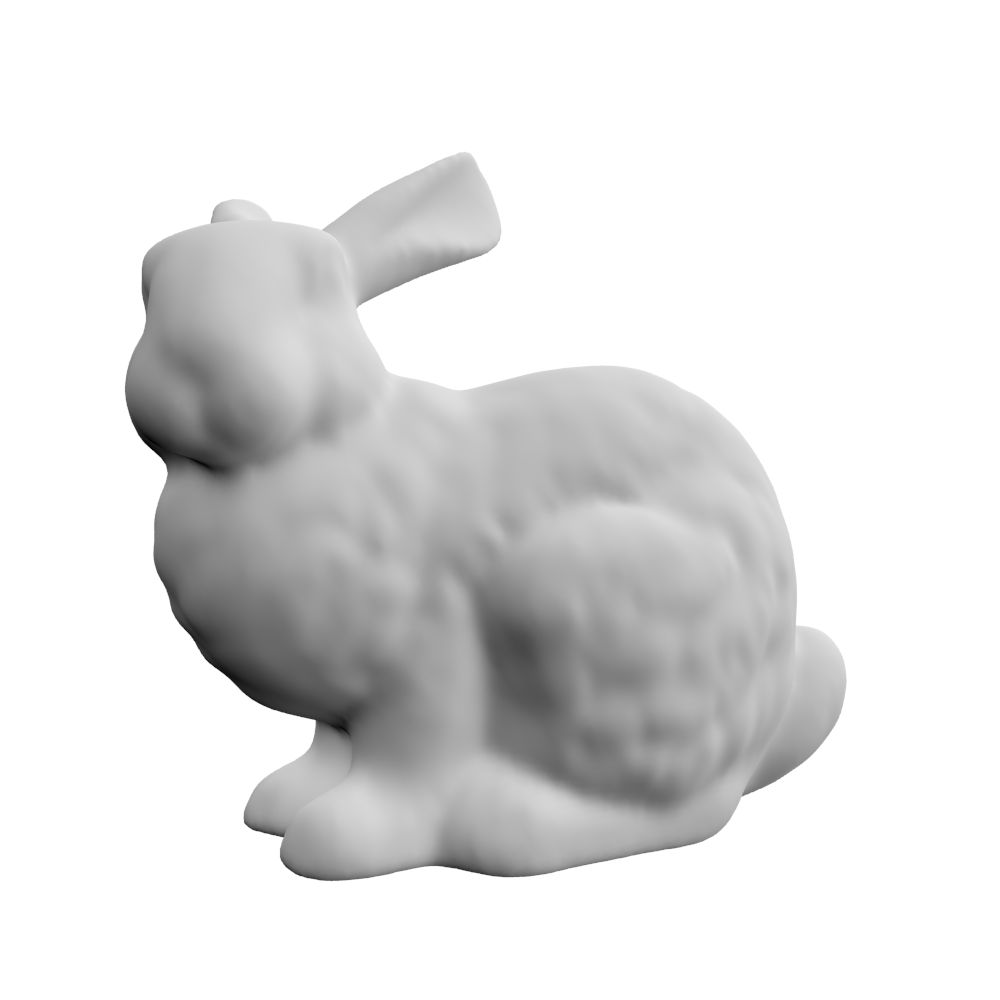
\includegraphics[width=\linewidth]{media/diffuse_bunny.png}
		\caption*{Lambert \ac{BRDF}}
	\end{subfigure}%
	\begin{subfigure}[t]{0.33\textwidth}
		\centering
		\captionsetup{justification=centering}
		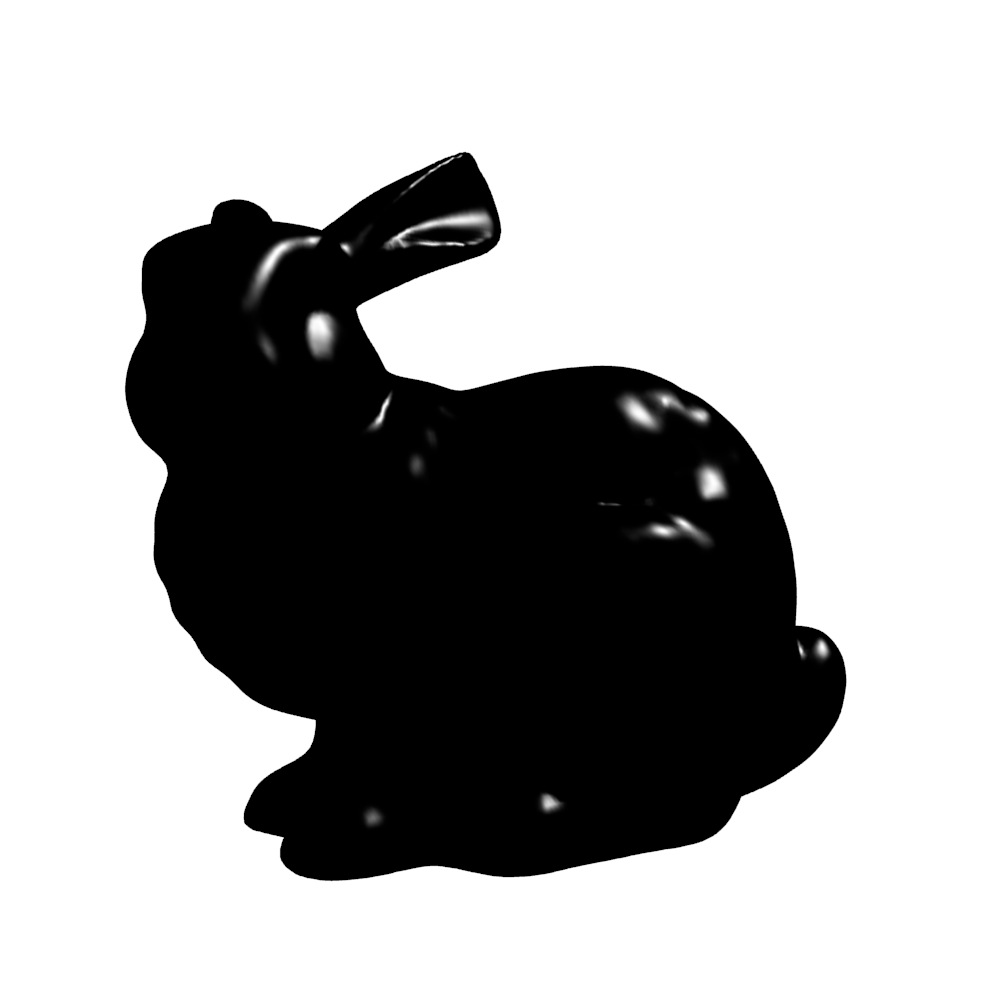
\includegraphics[width=\linewidth]{media/specular_bunny.png}
		\caption*{Blinn-Phong \ac{BRDF}\\ especular}
	\end{subfigure}%
	\begin{subfigure}[t]{0.33\textwidth}
		\centering
		\captionsetup{justification=centering}
		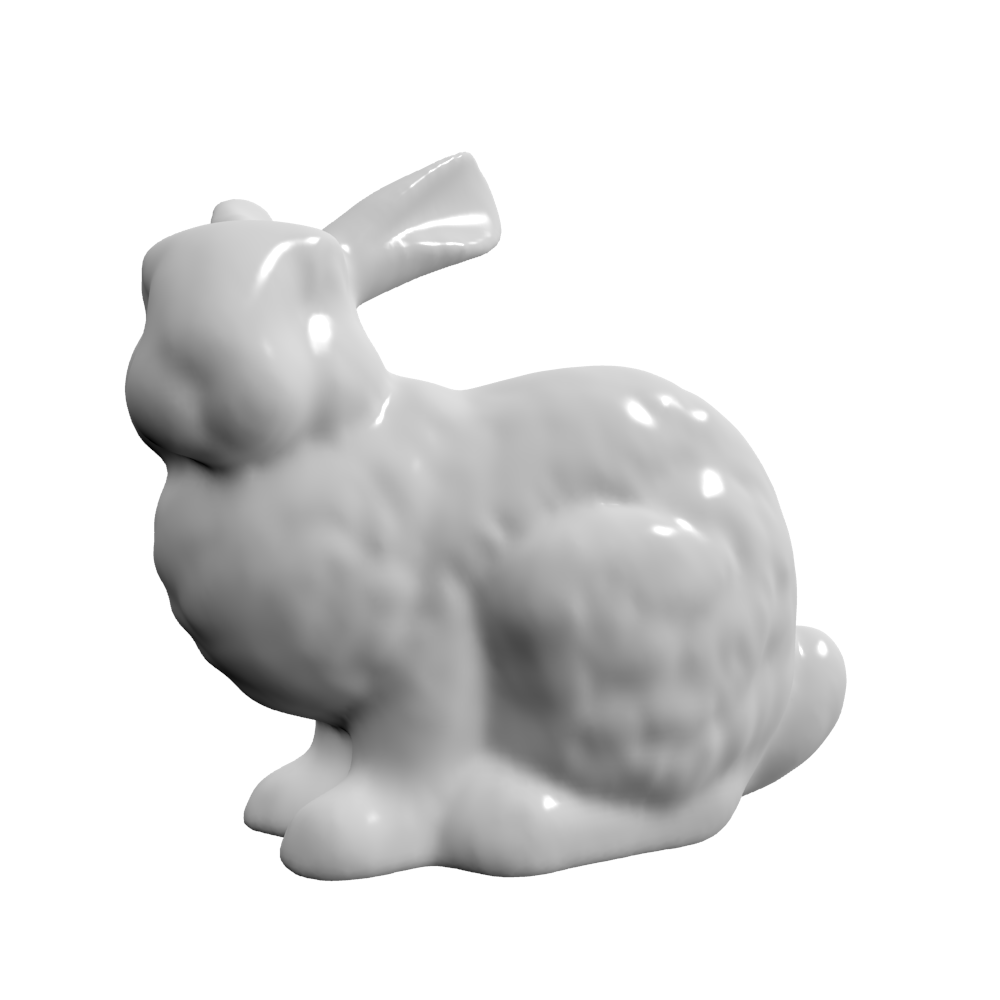
\includegraphics[width=\linewidth]{media/diffuse_specular_bunny.png}
		\caption*{Lambert \ac{BRDF} y \\Blinn-Phong \ac{BRDF} especular.}
	\end{subfigure}
	\caption{Ejemplo de \ac{BRDF}s. Se observa como estas afectan la apariencia final de la superficie.}
	\label{fig:brdfs_comparison}
\end{figure}

\subsection{Función de Distribución Normal}
La \ac{NDF} introducida por Alain Fournier \cite{fournier1992d} describe la densidad de las normales como una función de dirección. Funciones gaussianas como la siguiente es una de las posibles formas de una \ac{NDF}.
\begin{equation}
    f(x) = \frac{1}{\sigma\sqrt{2\pi}}e^{-\frac{(x-\mu)^2}{2\sigma^2}}
    \label{eq:ndf_ex1}
\end{equation}

En la función gaussiana el termino $\sigma^2$ es llamado variancia y el termino $\mu$ es llamado media. Tanto el producto como la convolución de dos distribuciones gaussianas es también una distribución gaussiana \cite{tina-2003}.

La función gaussiana puede ser utilizada como una representación direccional. En este caso la media es un vector promedio $D$ del lóbulo gaussiano. Como es descrito en el trabajo de Toksvig para el mipmapping de mapas de normales \cite{Toksvig05}, el valor de $\sigma$ puede ser calculado por la longitud del vector promedio $D$ utilizando la siguiente ecuación.
\begin{equation}
    \sigma^2 = \frac{1-|D|}{|D|}
    \label{eq:gaussia_eq}
\end{equation}
Esto permite obtener lóbulos gaussianos a partir de dos o más vectores para representar su dirección en común.

\begin{figure}[H]
	\centering
	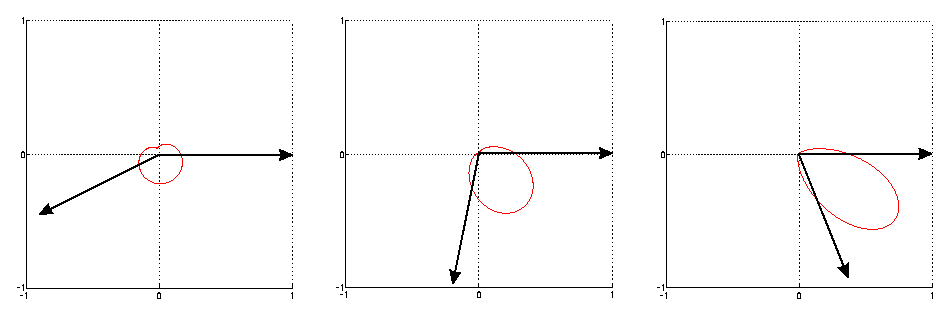
\includegraphics[width=0.85\linewidth]{media/lobes.eps}
	\caption{Ejemplo de lóbulos gaussianos según dos vectores, se puede observar como la forma del lóbulo cambia según la dirección promedio.}
	\label{fig:lobes_example}
\end{figure}

Algunas \ac{BRDF} también pueden describirse como distribuciones gaussianas, las propiedades de producto y convolución se mantienen.

\begin{figure}[H]
	\centering
	\begin{subfigure}[t]{0.3\textwidth}
		\centering
		\captionsetup{justification=centering}
		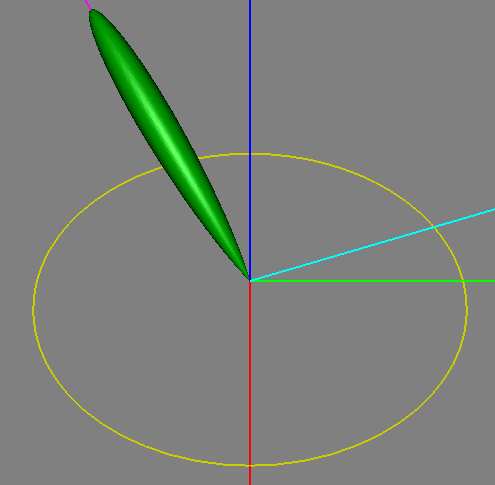
\includegraphics[width=\linewidth]{media/phong_lobule.png}
		\caption*{\ac{BRDF} Phong}
	\end{subfigure}\hfill
	\begin{subfigure}[t]{0.35\textwidth}
		\centering
		\captionsetup{justification=centering}
		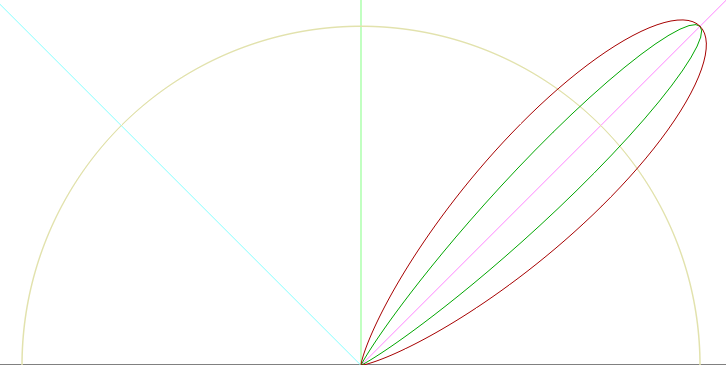
\includegraphics[width=\linewidth]{media/BlinnPhonglobules.png}
		\caption*{Gráfica de ambas en coordenadas polares.}
	\end{subfigure}\hfill
	\begin{subfigure}[t]{0.3\textwidth}
		\centering
		\captionsetup{justification=centering}
		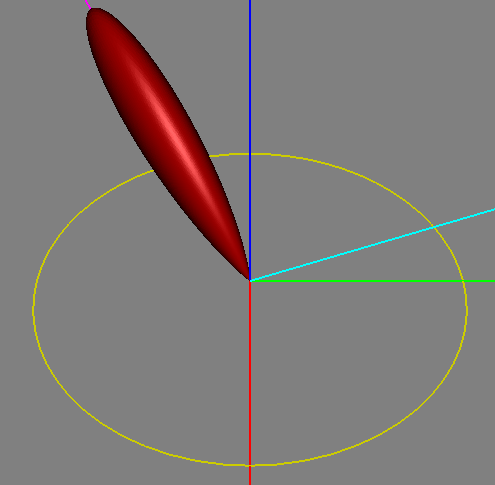
\includegraphics[width=\linewidth]{media/blinnphong_lobule.png}
		\caption*{\ac{BRDF} Blinn-Phong}
	\end{subfigure}\hfill
	\caption{Lóbulos especulares para BRDF Phong y Blinn-Phong para un $\Theta$ y $\Psi$ de $\angle 45$, se puede observar cómo estas describen la distribución de la dirección de reflectancia. Como se explica en \ref{para:blinn_phong} el valor de $n$ afecta la forma del lóbulo mientras mayor es este número más fino y largo es el lóbulo especular. Imágenes renderizadas en Disney's BRDF Explorer \cite{brdf_explorer}.}
	\label{fig:brdf_lobules}
\end{figure}
